 
 %\setcounter{page}{45}
 \clearpage
 %\pagenumbering{arabic}
 \newpage
 % \addcontentsline{toc}{chapter}{\hfill 34}
 \addtocontents{toc}{\protect\contentsline{chapter}{CAPÍTULO IV. Propuesta de diseño   \hfill  83}{}{}}
 
 

 \begin{titlepage}
 	
 	
 	\centering
 	\begin{tikzpicture}%opacity=0.5
 		\node[inner sep=0pt, ] (image) at (0,0) {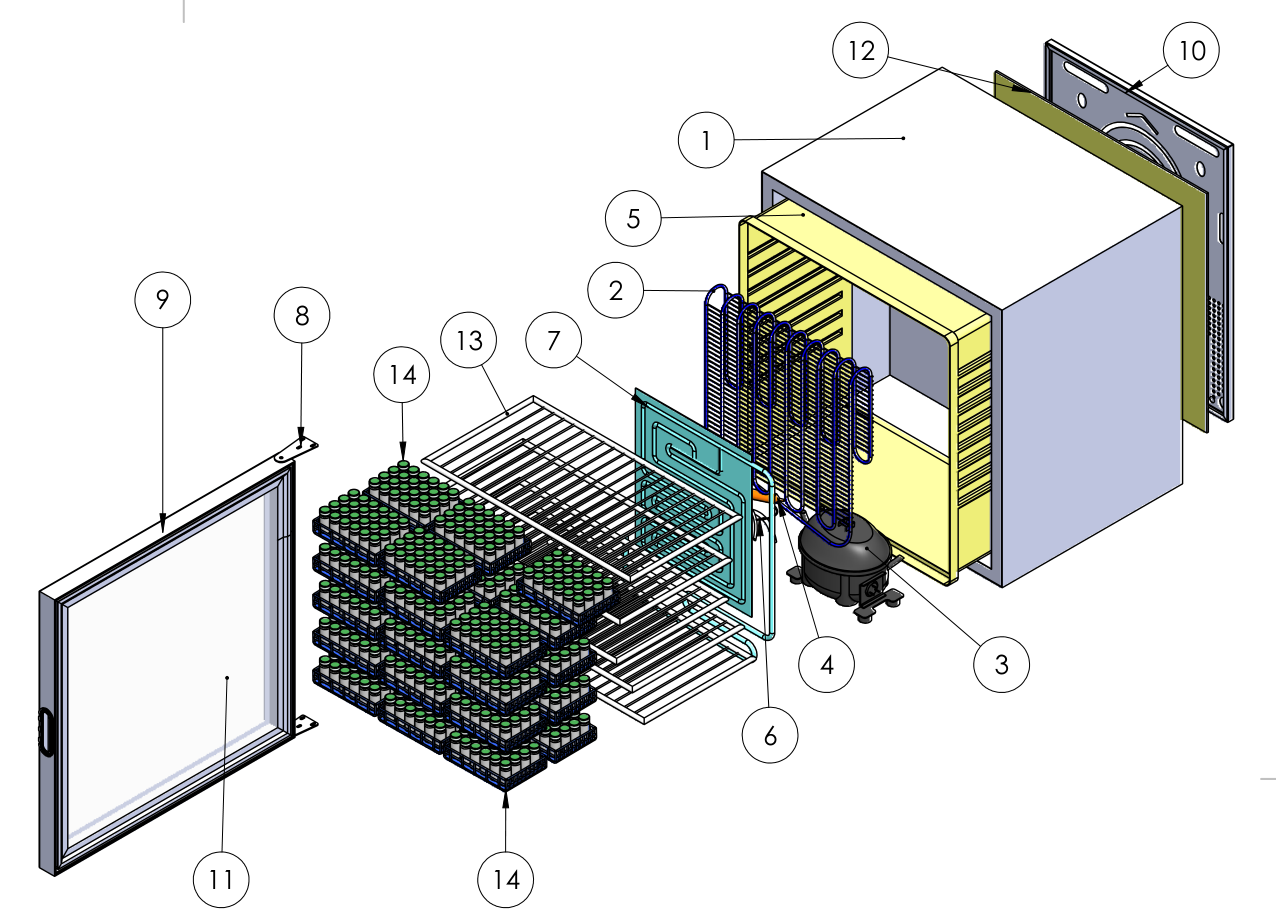
\includegraphics[width=\textwidth]{figures/front-chapetr4}};
 		\fill [white,path fading=south] (-5,-4) rectangle (5,4);
 		\node[black,font=\Huge\bfseries] at (0,3) {Capítulo V. Análisis de costos del proyecto};
 		\node[black,font=\Large\bfseries] at (0,1) {Estudio de costos del proyecto};
 		\node[black,font=\Large\bfseries] at (0,0) {Costos directos};
 		\node[black,font=\Large\bfseries] at (0,-1) {Estimación del costo del proyecto};
 	\end{tikzpicture}
 \end{titlepage}
 
 
 \newpage 
 
 \section*{Introducción}
 
 

 \setcounter{chapter}{5}
 \setcounter{page}{111}   
 \setcounter{section}{0}
 \setcounter{figure}{0}
 \setcounter{table}{0}
  \addcontentsline{toc}{section}{{Introducción}} 
La distribución de la cámara de refrigeración se detalla en la Figura \ref{fig:4.1}. El contenedor del refrigerador está adaptado con láminas compuestas de poliuretano (película interna fi - Poliuretano - película externa fe) en las cuatro paredes, con el objetivo de minimizar la pérdida de temperatura por transferencia térmica a través de las superficies. Esta aislación contribuye a evitar el uso de ventiladores, mejorando la eficiencia energética en las etapas iniciales del funcionamiento.

En la parte posterior de la cámara se integra la unidad de refrigeración, cuya función es proteger los componentes del sistema. Esta unidad alberga los elementos principales, como el compresor, el condensador y el dispositivo de expansión, que están conectados directamente al evaporador. El evaporador está situado en el interior de la cámara y conectado al serpentín, cuya función es asegurar una mejor distribución del refrigerante dentro de la cámara, lo que permite una disipación de calor más eficiente y uniforme.

Además, la cámara está equipada con diversas tapas y una cubierta de cristal, diseñadas para mantener el medicamento en condiciones óptimas de almacenamiento.

La cámara tiene dimensiones de 60 × 60 × 51.2 centímetros. Es fundamental considerar aspectos como el flujo de aire interno y la distribución térmica. La selección del serpentín garantizará una transferencia de calor eficiente y uniforme, minimizando las zonas frías o calientes que podrían afectar la integridad del producto. Además, en los cálculos de secciones posteriores se considera la capacidad del evaporador para manejar la carga térmica en función de la cantidad y tipo de insulina almacenada, así como las condiciones ambientales externas propias de la Alcaldía.

 \section{Costos Directos}
 Son aquellos costos que tienen una conexión directa con el proyecto y se reflejan de manera tangible; se manifiestan en el desarrollo del proyecto y en la conclusión de este. Son los costos responsables de manifestar de manera tangible aquello que en su principio fue una propuesta de solución, tanto en los componentes de la obra, como en los operadores responsables del desarrollo del proyecto.
 
 \subsection{Mano de obra}
 Para el desarrollo del proyecto se necesita de apoyo técnico y personal capacitado para la ejecución e instalación de componentes específicos. En este proyecto, es fundamental contar con técnicos especializados para la instalación de la unidad de refrigeración, cuyo sistema garantizará la correcta refrigeración del medicamento en cuestión, y debe estar adaptado a las necesidades específicas del entorno de almacenamiento.
 
 
 Según las tarifas estimadas por el Gobierno de México y la Secretaría de Economía del México, los técnicos especializados en instalación de sistemas de refrigeración tienen un salario aproximado de \$10,250.00 MXN por instalación. Este cálculo proviene de fuentes especializadas en la instalación y puesta en marcha de sistemas de refrigeración, y se estima que el tiempo necesario para la instalación de todos los componentes, incluidos los trabajos de aislamiento, es de aproximadamente 2,400 minutos, lo que equivale a un tiempo máximo de trabajo de 5 días.
OA 
 \subsection{Unidad Condensadora}
 La selección de la unidad condensadora toma en cuenta los siguientes parámetros esenciales para el correcto funcionamiento del sistema de refrigeración en la cámara destinada al almacenamiento de insulina:
 
 \begin{itemize}
 	\item \textbf{Carga térmica:} 2.8732 T.R. = 31,605.2724 BTU/h
 	\item \textbf{Temperatura de almacenamiento:} -18 °C (-0.4 °F)
 	\item \textbf{Temperatura de evaporación del refrigerante:} -40 °C (-40 °F)
 	\item \textbf{Temperatura del exterior:} 41 °C (105.8 °F)
 	\item \textbf{Temperatura de condensación del refrigerante:} 35 °C (95 °F)
 \end{itemize}
 
 Además de estos parámetros, es necesario considerar el tipo de refrigerante que emplea la unidad, ya que es el fluido de trabajo con el que opera todo el sistema. Se opta por el refrigerante R-404A, ya que este es el que maneja la unidad evaporadora, lo que garantiza la compatibilidad y eficiencia en el sistema de refrigeración.
 
 Es importante destacar que la elección de la unidad condensadora y el refrigerante deben ser coherentes con las condiciones operativas de la cámara de refrigeración y la carga térmica que se manejará, para evitar fluctuaciones de temperatura que puedan comprometer la efectividad del almacenamiento del medicamento.
 
 \section{Distribución y Características de la Cámara de Refrigeración}
 La cámara de refrigeración se encuentra diseñada para mantener las condiciones óptimas para el almacenamiento de insulina. La distribución del espacio y los componentes de la cámara se detallan en la figura 4.1, destacando el uso de láminas compuestas de poliuretano para minimizar la pérdida de temperatura por transferencia térmica. Estas láminas están ubicadas en las cuatro paredes de la cámara, lo que contribuye a evitar el uso de ventiladores y mejora la eficiencia energética en las etapas iniciales del funcionamiento.
 
 \subsection{Unidad de Refrigeración}
 En la parte posterior de la cámara, se integra la unidad de refrigeración, cuya función es proteger los componentes del sistema. Esta unidad alberga los elementos principales, como el compresor, el condensador y el dispositivo de expansión, los cuales están conectados directamente al evaporador. El evaporador está ubicado en el interior de la cámara y conectado al serpentín, que asegura una distribución adecuada del refrigerante dentro de la cámara, permitiendo una disipación de calor más eficiente y uniforme.
 
 \subsection{Consideraciones del Producto}
 Las dimensiones de la cámara son 60 × 60 × 51.2 centímetros, lo que permite una distribución eficiente del aire y una distribución térmica adecuada. En este sentido, la selección del serpentín será clave para garantizar una transferencia de calor eficiente y minimizar las zonas frías o calientes que podrían afectar la integridad del producto. Además, la capacidad del evaporador se seleccionará en función de la carga térmica generada por la cantidad y tipo de insulina almacenada, así como las condiciones ambientales externas propias de la Alcaldía de Azcapotzalco.
 
 \section{Ubicación Geográfica}
 Es importante considerar las condiciones geográficas y climáticas del lugar en donde estará ubicada la cámara de refrigeración. En este proyecto, se toma como referencia el Pueblo de Santa Bárbara, en la Alcaldía Azcapotzalco, Ciudad de México. Las condiciones climáticas en la zona se resumen a continuación:
 
 \begin{itemize}
 	\item \textbf{Temperatura de bulbo seco:} 25 °C (77 °F)
 	\item \textbf{Temperatura de bulbo húmedo:} 20 °C (68 °F)
 	\item \textbf{Altitud:} 2,240 msnm
 	\item \textbf{Presión atmosférica:} 1,023 Pa (1 atm)
 \end{itemize}
 
 \section{Condiciones del Producto a Refrigerar}
 La insulina debe ser almacenada en un rango de temperatura específico para garantizar su efectividad. Según las condiciones proporcionadas por la UMF.40, las condiciones de almacenamiento para la insulina son las siguientes:
 
 \begin{table}[h!]
 	\centering
 	\caption{Condiciones del Producto a Refrigerar}
 	\begin{tabular}{|c|c|c|c|}
 		\hline
 		\textbf{Producto} & \textbf{Temp. Almacenamiento (°C)} & \textbf{Humedad relativa (\%)} & \textbf{Vida aprox. (días)} \\ \hline
 		Insulina & 2 - 8 & 35 - 70 & 28 (antes de abrir) \\ \hline
 	\end{tabular}
 \end{table}
 
 En cuanto al tipo de insulina, se proporcionan dos tipos de insulina a los pacientes diabéticos: \textit{Humalog Insulina Lispro} y \textit{Insulina Lantus}. Ambos productos son suministrados por el gobierno, lo que garantiza que su logística de cadena de suministro está debidamente regulada.
 
 
 \section{Comparación de Unidades Condensadoras Thermo King}
 El análisis a continuación presenta las características y ventajas de las unidades condensadoras tipo Thermo King, comparando tres opciones disponibles para la refrigeración en la UMF40. La elección de la unidad adecuada dependerá de varios factores, como la carga térmica necesaria, el costo y la facilidad de mantenimiento.
 
 \begin{table}[h!]
 	\centering
 	\caption{Comparación de Unidades Condensadoras Tipo Thermo King}
 	\begin{tabular}{|c|c|c|c|c|}
 		\hline
 		\textbf{Opción} & \textbf{Proveedor/Marca} & \textbf{Ventajas} & \textbf{Desventajas} & \textbf{Costo} \\ \hline
 		A-500 & Thermo King & Cumple con la carga térmica necesaria. Facilidad de mantenimiento. Supervisor de consumo de combustible. Silencioso. & Costo elevado. El deshielo eléctrico aumenta la carga térmica. & \$53,024.57 USD \\ \hline
 		A-500 Whisper Pro & Thermo King & Fácil mantenimiento. Silencioso. Uso fácil. & No cumple con la carga térmica requerida. Costo elevado comparado con su utilidad. & \$64,789.26 USD \\ \hline
 		A-500 Spectrum & Thermo King & Menor tiempo de desescarche. Bajo precio. & No tiene seguimiento de consumo de combustible. & \$72,795.00 USD \\ \hline
 	\end{tabular}
 \end{table}
 
 \subsection{Análisis de las Opciones}
 Cada una de las opciones presenta características particulares que pueden ser relevantes dependiendo de las necesidades específicas del proyecto en la UMF40. Se debe considerar que el costo es un factor importante, pero también lo es la eficiencia en el mantenimiento y la capacidad de enfriamiento.
 
 \begin{itemize}
 	\item \textbf{A-500 Thermo King:} Es la opción que mejor cumple con la carga térmica necesaria para el almacenamiento de insulina en la UMF40. A pesar de su costo elevado, se destaca por su fácil mantenimiento y el control del consumo de combustible.
 	\item \textbf{A-500 Whisper Pro:} Aunque es silenciosa y de fácil uso, no cumple con los requerimientos de carga térmica. Su costo también es elevado en relación con su utilidad, lo que puede hacerla menos atractiva para este tipo de proyecto.
 	\item \textbf{A-500 Spectrum:} Ofrece un menor tiempo de desescarche y un precio más bajo, pero carece de la funcionalidad de seguimiento del consumo de combustible, lo que podría ser un inconveniente en términos de eficiencia energética.
 \end{itemize}
 
 \subsection{Preferencia y Elección}
 La elección final dependerá de los requisitos específicos de refrigeración, así como del presupuesto disponible para la unidad condensadora. Basado en la carga térmica necesaria y la eficiencia del mantenimiento, la opción \textbf{A-500 Thermo King} sería la preferida, con una valoración d
 
 
 
 
 
 
 
 
  
%  \begin{center}
% 	\begin{tikzpicture}
%  		% Principio 1 - Desarrollar las alternativas
%  		\node[draw, rounded corners, fill=blue!10, minimum width=8cm, minimum height=2cm] (p1) at (0,0) {
%  			\faLightbulb[regular] \textbf{ PRINCIPIO 1 — DESARROLLAR LAS ALTERNATIVAS} \\
%  			
%  			La selección (decisión) se da entre alternativas. Las alternativas necesitan identificarse y luego definirse para utilizarse en el análisis posterior.
%  		};
%  		
%  		% Principio 2 - Centrarse en las diferencias
%  		\node[draw, rounded corners, fill=green!10, minimum width=8cm, minimum height=2cm, below=of p1] (p2) {
%  			\faExchangeAlt \textbf{ PRINCIPIO 2 — CENTRARSE EN LAS DIFERENCIAS} \\
% 			
%  			Sólo las diferencias entre los resultados esperados en las alternativas son relevantes para su comparación, y deben tomarse en cuenta en la decisión.
%  		};
%  		
%  		% Principio 3 - Punto de vista consistente
%  		\node[draw, rounded corners, fill=orange!10, minimum width=8cm, minimum height=2cm, below=of p2] (p3) {
%  			\faEye \textbf{ PRINCIPIO 3 — UTILIZAR UN PUNTO DE VISTA CONSISTENTE} \\
%  			
%  			Los resultados futuros de las alternativas deben desarrollarse en forma consistente a partir de un punto de vista definido.
%  		};
%  		
%  		% Principio 4 - Unidad de medida común
%  		\node[draw, rounded corners, fill=purple!10, minimum width=8cm, minimum height=2cm, below=of p3] (p4) {
%  			\faBalanceScale \textbf{ PRINCIPIO 4 — USAR UNA UNIDAD DE MEDIDA COMÚN} \\
%  			
%  			El uso de una unidad de medida común para numerar tantos resultados futuros como sea posible, simplificará el análisis.
%  		};
%  		
%  		% Principio 5 - Criterios relevantes
%  		\node[draw, rounded corners, fill=red!10, minimum width=8cm, minimum height=2cm, below=of p4] (p5) {
%  			\faCheck \textbf{ PRINCIPIO 5 — TOMAR EN CUENTA TODOS LOS CRITERIOS RELEVANTES} \\
%  			
%  			La selección de la alternativa requiere el uso de un criterio y debe considerar tanto resultados numéricos como descriptivos.
%  		};
%  		
%  		% Principio 6 - Incertidumbre explícita
%  		\node[draw, rounded corners, fill=yellow!10, minimum width=8cm, minimum height=2cm, below=of p5] (p6) {
%  			\faExclamationTriangle \textbf{ PRINCIPIO 6 — HACER EXPLÍCITA LA INCERTIDUMBRE} \\
%  			La incertidumbre es inherente a los resultados futuros y debe reconocerse en el análisis.
%  		};
%  		
  		% Principio 7 - Revisar decisiones
%  		\node[draw, rounded corners, fill=teal!10, minimum width=8cm, minimum height=2cm, below=of p6] (p7) {
%  			\faRedo \textbf{ PRINCIPIO 7 — REVISAR LAS DECISIONES} \\
%  			La mejora del proceso de decisiones surge de un proceso adaptativo comparando resultados proyectados y reales.
%  		};
%  		
%  		% Flechas entre los principios
%  		\foreach \i in {1,...,6}
%  		\draw[->, thick] (p\i.south) -- (p\the\numexpr\i+1.north);
%  		
%  	\end{tikzpicture}
%  \end{center}

  
  
  
  
  
  
  
  